\chapter{Stand van zaken}
\label{ch:stand-van-zaken}

% Tip: Begin elk hoofdstuk met een paragraaf inleiding die beschrijft hoe
% dit hoofdstuk past binnen het geheel van de bachelorproef. Geef in het
% bijzonder aan wat de link is met het vorige en volgende hoofdstuk.

% Pas na deze inleidende paragraaf komt de eerste sectiehoofding.

%Dit hoofdstuk bevat je literatuurstudie. De inhoud gaat verder op de inleiding, maar zal het onderwerp van de bachelorproef *diepgaand* uitspitten. De bedoeling is dat de lezer na lezing van dit hoofdstuk helemaal op de hoogte is van de huidige stand van zaken (state-of-the-art) in het onderzoeksdomein. Iemand die niet vertrouwd is met het onderwerp, weet er nu voldoende om de rest van het verhaal te kunnen volgen, zonder dat die er nog andere informatie moet over opzoeken \autocite{Pollefliet2011}.
%
%Je verwijst bij elke bewering die je doet, vakterm die je introduceert, enz. naar je bronnen. In \LaTeX{} kan dat met het commando \texttt{$\backslash${textcite\{\}}} of \texttt{$\backslash${autocite\{\}}}. Als argument van het commando geef je de ``sleutel'' van een ``record'' in een bibliografische databank in het Bib\TeX{}-formaat (een tekstbestand). Als je expliciet naar de auteur verwijst in de zin, gebruik je \texttt{$\backslash${}textcite\{\}}.
%Soms wil je de auteur niet expliciet vernoemen, dan gebruik je \texttt{$\backslash${}autocite\{\}}. In de volgende paragraaf een voorbeeld van elk.
%
%\textcite{Knuth1998} schreef een van de standaardwerken over sorteer- en zoekalgoritmen. Experten zijn het erover eens dat cloud computing een interessante opportuniteit vormen, zowel voor gebruikers als voor dienstverleners op vlak van informatietechnologie~\autocite{Creeger2009}.

 Dit hoofdstuk is de aanloop naar wat serverless is en wat het inhoudt. Er wordt vertrokken vanuit enkele basisprincipes omtrent cloud computing die de lezer meer inzicht geven in dit onderwerp. Lezers die nog weinig tot geen kennis hebben vinden hier voldoende informatie om een beeld te vormen bij cloud computing concepten alsook serverless. Lezers die vertrouwd zijn met cloud computing en op de hoogte zijn van de basisconcepten kunnen meteen verdergaan naar sectie \ref{sec:wat-is-serverless}, hoewel deze inleiding een goede opfrissing kan zijn.
 
\section{Wat is Cloud computing?}
\label{sec:wat-is-cloud-computing}
 
Cloud computing is alomtegenwoordig en een basiskennis van het begrip is interessant voor iedereen die werkt binnen de IT wereld. In dit hoofdstuk worden allerhande begrippen over cloud computing geïntroduceerd. Na het lezen van dit hoofdstuk zal u instaat zijn om mee te praten over de basiscomponenten en workflows binnen cloud computing. De begrippen in dit hoofdstuk zijn van belang voor het vervolg van dit onderzoek naar serverless of FaaS.

\subsection{Definitie}

Cloud computing is:
\newline
On-demand computing services die worden aangeboden via het internet. Deze services omvatten onder andere servers, databanken, netwerkfuncties, opslag en nog veel meer. Werken in de cloud volgt het uitgangspunt: je betaalt voor wat je gebruikt. De cloud biedt flexibiliteit, schaalbaarheid en snelle provisioneer tijd. Het stelt bedrijven instaat benodigde IT infrastructuur uit te besteden en zo dus ook geld te besparen. In de cloud is het mogelijk om up- en down te schalen naargelang de huidige noden, de cloud is met andere woorden elastisch. \autocite{Davis2017}
\newline
\newline
Deze definitie vormt een algemene omschrijving van wat cloud computing allemaal kan inhouden. Het is zinvol om deze definitie te gebruiken als uitgangspunt om cloud computing verder in detail te omschrijven.

\subsection{Inleiding}
Het internet en de IT-wereld transitioneert en evolueert enorm snel. Klassieke IT infrastructuur die werkt volgens het client-server principe maakt de transitie naar een cloudgebaseerde benadering. In een klassieke infrastructuur benadering koopt een bedrijf zelf servers aan, installeert en onderhoudt deze. Een bedrijf moet in dit opzicht alles voorzien: datacenter, netwerk, elektriciteit, beveiliging, ... . Een eigen infrastructuur onderhouden in een opgezet datacenter brengt een grote kost met zich mee. Voor de huidige datacenter infrastructuren werden er vaak voor alle applicaties aparte servers voorzien. Er draaide toen één applicatie op één fysieke machine. De traditionele architectuur bracht grote kosten met zich mee en resulteerde vaak ook dat er op sommige momenten te veel resources waren in vergelijking met hoeveel men er maar nodig had. De klassieke benadering heeft dus heel wat beperkingen. 
\newline
\newline
Later, in 1999 introduceerde VMware als eerste een nieuw product: VMware Virtual Platform, virtualisatie was geboren. Virtualisatie zorgt ervoor dat bovenop de hardware van de server een "hypervisor" kan worden geïnstalleerd. Een hypervisor is een programma dat toelaat om een server onder te verdelen in meerdere servers met elk hun eigen besturingssysteem. In de traditionele benadering werd er voor elke legacy-applicatie één server met één OS voorzien. Met gebruik van virtualisatie is het dus mogelijk om meerdere aparte servers te migreren naar één fysieke machine waarop een hypervisor draait. Dankzij de hypersvisor draaien meerdere servers nog steeds onafhankelijk van elkaar op hun eigen besturingssysteem op dezelfde fysieke hardware. Virtualisatie zorgt ervoor dat er minder fysieke servers moeten worden aangekocht, wat de kost dus aanzienlijk vermindert. Binnen virtualisatie kunnen ook complexe netwerken worden gebouwd zodat gevirtualiseerde servers met elkaar en de buitenwereld kunnen communiceren. \autocite{RedHat2019}. In 
figuur ~\ref{fig:klassiek-vs-virtualisatie} wordt het verschil tussen een klassieke server met één OS en één applicatie vergeleken met een server waarop gevirtualiseerde servers draaien. Virtualisatie is een van de grondslagen van cloud computing, deze technologie maakt het vandaag de dag mogelijk om infrastructuur te draaien in de cloud.
\newline
\newline
\begin{figure}
    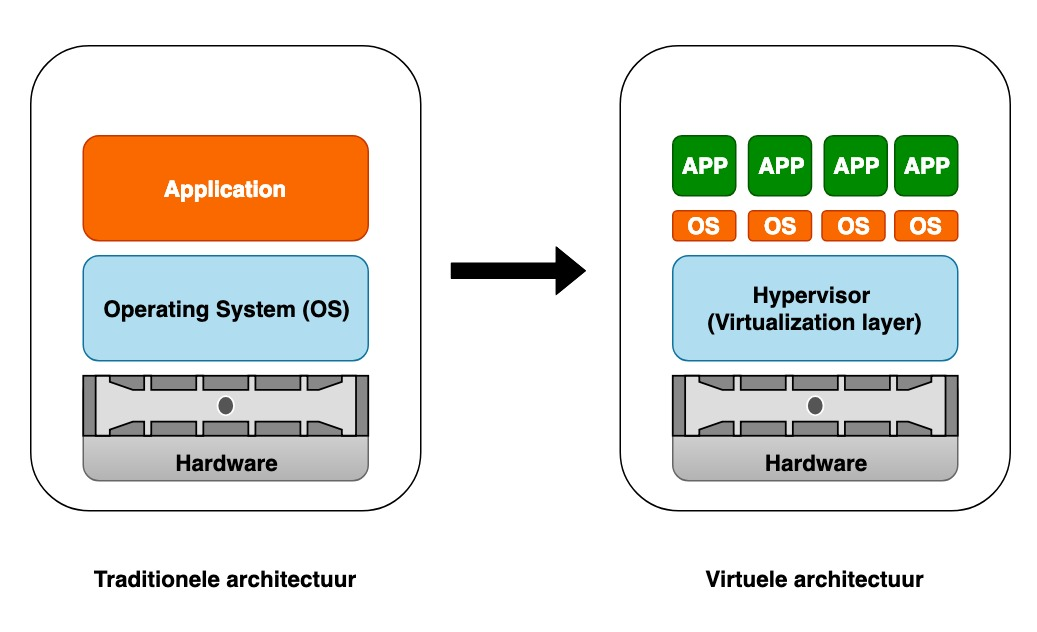
\includegraphics[width=1\textwidth]{img/klassiek_virtualisatie}
    \caption{De architectuur aan de linkerkant weergeeft een beeld van hoe het traditionele server architectuur model eruitziet. De afbeelding rechts toont hoe een gevirtualiseerde architectuur eruitziet.} 
    \label{fig:klassiek-vs-virtualisatie}  
\end{figure}
\newline

Wanneer er naar de cloud gerefereerd wordt, dan bedoelt men meestal de cloud services die grote providers als een Google, Amazon en Microsoft aanbieden. Laten we de conventie maken dat wanneer er in de inleiding gerefereerd wordt naar de cloud, dit wijst op de cloud services die door cloud providers worden aangeboden. Later maken we de distinctie tussen welke verschillende soorten cloud er zijn, met elk hun eigenschappen. De afgelopen jaren hebben steeds meer bedrijven gekozen om hun applicaties en infrastructuur naar de cloud te migreren. Migratie naar de cloud is interessant in verschillende opzichten, er zijn heel wat voordelen aan verbonden die in sectie ~ref{voor-en-nadelen} worden uitgelegd. De grootste motivatie waarom bedrijven naar de cloud migreren is enerzijds het feit dat er enkel betaald wordt voor wat men verbruikt en anderzijds neemt het heel wat overhead zoals het onderhouden van infrastructuur weg. Cloud computing zorgt ervoor dat gebruikers een gedeelde bron van resources en opslag kunnen gebruiken bij een cloud provider. Een poel of bron van resources kan worden gezien als duizenden servers waarop virtuele machines of applicaties draaien. Deze services worden verschaft via het internet. Gebruikers betalen enkel voor de resources die ze verbruiken, zo worden de kosten meestal berekend op de tijd die een server draait en welke gespecificeerde resources deze verbruikt. Een model waarin enkel betaald wordt voor het het verbruik wordt ook wel het "Pay as you go model" genoemd. De cloud is veelzijdig en biedt mogelijkheden op verschillende niveaus, deze worden in volgende onderdelen besproken. \autocite{Seghal2018} 


\subsection{Cloud types op deployment niveau}
\label{cloud-deployment-level}
De Cloud kan worden onderverdeeld in verschillende types op niveau van deployment. De onderverdeling op niveau van deployment slaat op de locatie waar de cloud infrastructuur draait, bijvoorbeeld in een datacenter van een grote cloud provider of bij een bedrijf op locatie in een eigen datacenter. Volgens \textcite{Goyal2014} kan de cloud worden opgedeeld in vier verschillende soorten met elk hun specifieke eigenschappen. Vooreerst wordt uitgelegd wat men bedoelt met on-premises infrastructuur.

\subsubsection{On-premises}
Een on-premises infrastructuur wijst op een IT infrastructuur die wordt beheerd door een organisatie zelf, de hardware bevinden zich ook op locatie bij het bedrijf. Een organisatie die over een on-premises of op locatie infrastructuur beschikt staat in voor het volledige beheer hiervan, dit gaat van fysieke installatie van hardware tot het beveiligen van applicatie op niveau van software. Een on-premises installatie zien we vaak terug in klassieke benaderingen of in bedrijven waar ze nog niet overtuigd zijn van het hele cloud gebeuren. Sommige organisaties kiezen nadrukkelijk om hun infrastructuur niet in de cloud te draaien om redenen gerelateerd aan privacy en confidentialiteit van data.

\subsubsection{Publieke cloud}
De publieke cloud wordt onderhouden door een derde partij. Publieke cloud providers bieden services en resources aan die op basis van een soort huurcontract geconsumeerd worden. Klanten die services of infrastructuur huren bij publieke cloud providers kunnen deze raadplegen via het internet. Publieke cloud services worden verschaft aan iedereen, ze zijn met andere woorden voor iedereen toegankelijk. De publieke cloud stelt organisaties instaat te besparen op aankoop van infrastructuur. Het is mogelijk om te betalen naargelang de resources of diensten die worden gebruikt. Dit is het selling point van de publieke cloud. Data die gemaakt of opgeslagen wordt door gebruikers bevindt zich ook in het datacenter van de cloud provider. Voorbeelden van publieke cloud providers zijn, zoals eerder al aangehaald, Google, Amazon en Microsoft.

\subsubsection{Private cloud}
Private cloud bestaat in verschillende vormen, het kan een datacenter zijn dat op locatie staat en onderhouden wordt of een cloud infrastructuur die is opgezet in een datacenter waar servers worden gehuurd. Een private cloud wordt door de organisatie zelf volledig onderhouden, er is ook enkel toegang voor de organisatie zelf of voor toegestane derde partijen. Wanneer er gekozen wordt voor een private cloud infrastructuur dan brengt dit de veelzijdigheid en tools van cloud computing met zich mee. Private cloud wordt vooral gekozen voor het waarborgen van privacy en veiligheid van data. Deze benadering wordt door veel bedrijven gekozen die veel confidentiële- en bedrijfskritische data moeten verwerken, denk maar aan banken, overheid en farmaceutica.

\subsubsection{Hybride cloud}
Een hybride cloud bestaat uit minstens één private en één publieke cloud. Wanneer verschillende soorten cloud met elkaar worden samengebracht wordt er verwezen naar een hybride cloud. Een hybride cloud wordt opgezet volgens verschillende standaarden en cloud- en hardware specifieke patenten. Een hybride cloud biedt de veelzijdigheid voor up- en down schaling zoals in de publieke cloud, en de veiligheid en integriteit zoals in de private cloud. Het implementeren van een hybride cloud omgeving is moeilijker omdat security hier heel wat overhead met zich meebrengt.

\subsubsection{Communtiy cloud}
Community cloud valt tussen de publieke en private cloud. Een community cloud bestaat uit twee of meer deelnemende partijen. Dit type van cloud valt te vergelijken met de private cloud die gedeeld wordt door meerdere partijen. Gebruik van een community cloud reduceert de aankoopkost van infrastructuur en de management kosten voor het opzetten van het cloud datacenter.


\subsection{Cloud service modellen}
\label{cloud-service-level}
Naast onderscheid op basis van de locatie waar cloud infrastructuur gedeployed wordt, maakt men ook onderscheid op niveau van service. Termen zoals PaaS, IaaS en SaaS horen tot deze sectie \autocite{Goyal2014}, in volgende drie secties worden deze veelvoorkomende klassieke cloud computing modellen samengevat.

\subsubsection{Infrastructure-as-a-Service (IaaS)}
Het IaaS service model biedt gebruikers computing, processing, networking en opslag aan waarop applicaties gedraaid kunnen worden. De gebruiker staat in voor het volledige beheer van de inrastructuur bovenop de aangeboden hardware. De componenten die aanpasbaar zijn, zijn onder andere het OS, de middleware, runtime, data en applicaties. De cloud provider staat in voor de networking, opslag, fysieke servers en bovenliggende virtualisatie. IaaS vormt de basis waarop Cloud computing is gebouwd, overige service modellen bouwen hierop ook verder. Gebruikers die controle willen hebben over (bijna) alle onderdelen van hun cloud infrastructuur opteren voor het gebruik van IaaS. Voorbeelden van IaaS zijn onder andere Google Cloud Platform Compute Engine, Amazon Web Services EC2 en Microsoft Azure.

\subsubsection{Platform-as-a-Service (PaaS)}
PaaS is vooral gericht op ontwikkelaars. Platform-as-a-Service stelt gebruikers instaat op een eenvoudige manier softwareapplicaties op te zetten zonder zorgen over de onderliggende infrastructuur. Cloud providers die PaaS diensten verschaffen staan in voor het volledige beheer van de infrastructuur zoals servers, zowel virtueel als fysiek, computing, opslag, netwerk, beveiliging, bijhorende tools en API's. Het beheer van servers zoals OS en dergelijke wordt ook door de cloud provider voorzien, PaaS voorziet een platform om applicaties op te draaien. Gebruikers staan enkel in voor ontwikkeling van de applicatie en de data die daar bijhoort. Als PaaS oplossing wordt vaak AWS Elastic Beanstalk gebruikt.

\subsubsection{Software-as-a-Service (SaaS)}
In het Software-as-a-Service model wordt de gehele infrastructuur, inclusief applicatie beheerd door de provider. SaaS voorziet applicaties die draaien in de cloud en raadpleegbaar zijn via een computer of mobiel apparaat, vaak simpelweg via een webbrowser. In het verleden moest software meestal worden aangekocht en worden geïnstalleerd op individuele systemen, SaaS is hiervoor de oplossing. Wanneer er gebruik wordt gemaakt van SaaS wordt de software aangerekend op basis van subscripties per gebruiker, dit kan op basis van tijd of verbruik. SaaS draait, zoals eerder gezegd, in de cloud en vereist dus geen extra installatie van software. Eén van de bekendste SaaS applicaties is Office 365, deze Microsoft services werken met een maandelijkse subscriptie die betaald wordt per gebruiker. Een voorbeeld van een gratis SaaS applicatie is bijvoorbeeld Google Docs.
\begin{figure}
    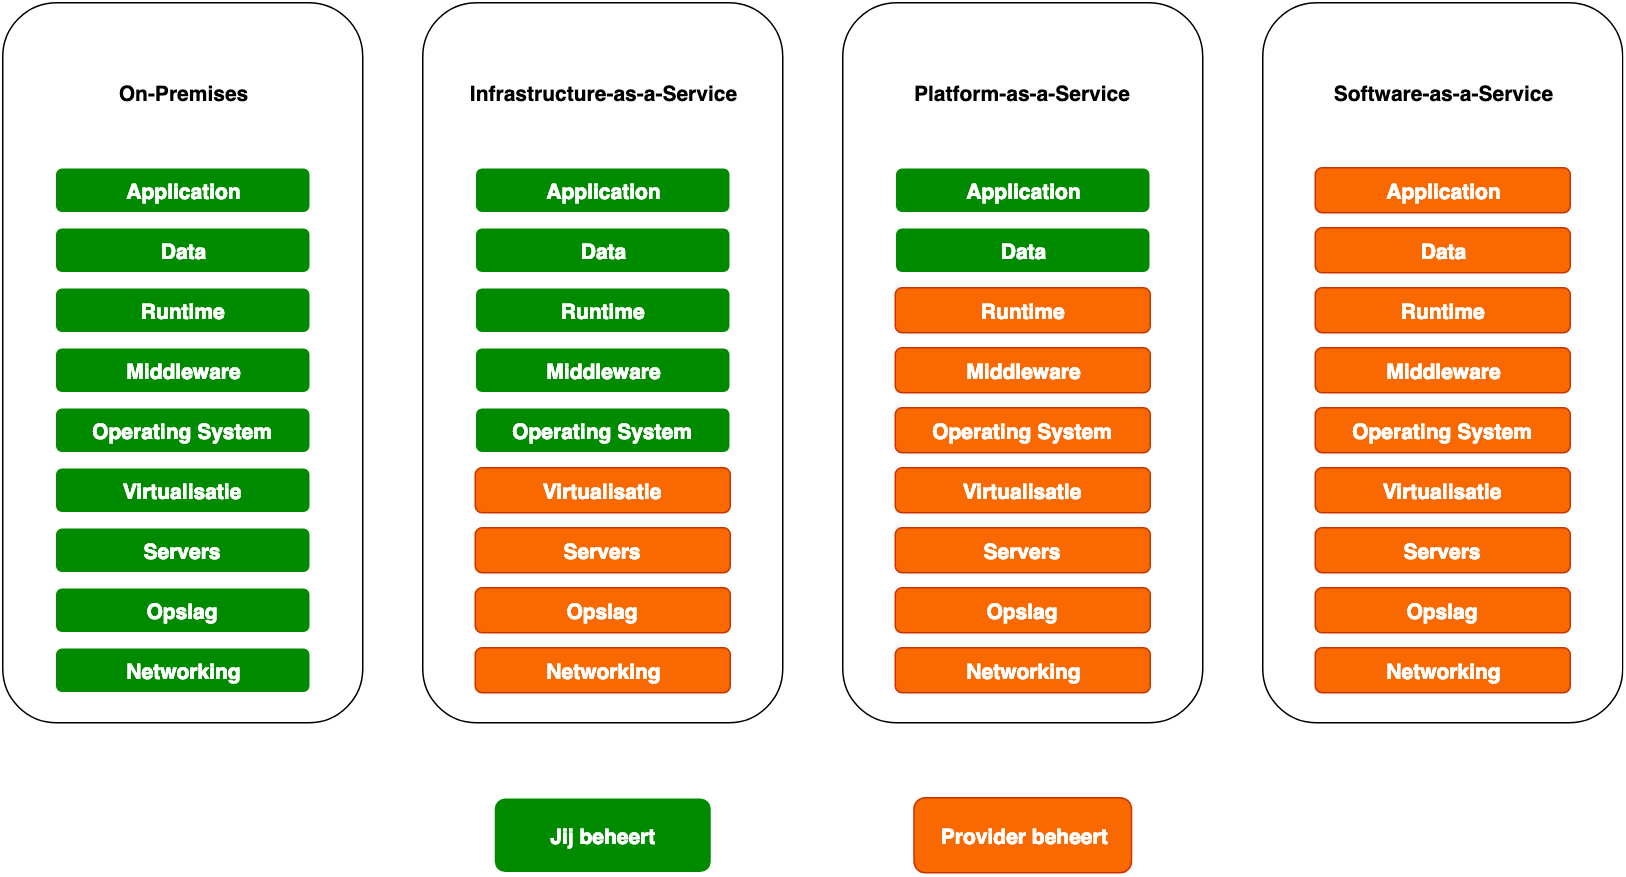
\includegraphics[width=1\textwidth]{img/cloud_service_level.png}
    \caption{De afbeelding weergeeft een schematische voorstelling van de verschillende cloud service niveaus. De groene kleur duidt alle onderdelen aan die zelf te managen zijn. De oranje kleur geeft aan welke onderdelen de cloud provider beheert.} 
    \label{fig:cloud-service-levels}  
\end{figure}
\newline

\subsection{Voor-en nadelen}
\label{voor-en-nadelen}
Cloud computing kent voordelen die heel wat mogelijkheden bieden ten opzichte van de klassieke benadering omtrent infrastructuur. \autocite{Azure2019} De voordelen zijn veelbelovend maar ook de nadelen mogen zeker niet over het hoofd worden gezien en dienen in kaart te worden gebracht om op de hoogte te zijn van mogelijke gevaren en bedreigingen.\autocite{Sosinsky2011} 

\subsubsection{Voordelen}

\begin{description}[style=unboxed, labelwidth=\linewidth, listparindent =0pt]
    \item[Lagere kosten]
    Cloud computing zorgt ervoor dat bedrijven zelf geen fysieke hardware meer hoeven aan te kopen voor hun eigen datacenter om software en applicaties te draaien. Een bedrijf hoeft bijvoorbeeld zelf geen webserver meer aan te kopen en te installeren om een webapplicatie te kunnen draaien, de benodigde hardware is beschikbaar bij verschillende cloud providers. Daarnaast zijn er ook geen kosten voor elektriciteitsvoorzieningen. De enige kost zijn de prijzen die de cloud provider aanrekent om de apparatuur of diensten ter beschikking te stellen.
    \newline

    \item[Performantie]
    Datacenters van grote cloud providers bevinden zich verspreid doorheen de hele wereld. De verspreiding van datacenters zorgt voor een lage latency en zorgt ervoor dat werken in de cloud voelt alsof de server in het eigen bedrijf staat. Computing componenten worden ook geregeld geüpgrade naar de laatste versies zodat de performantie verzekerd kan worden.
    \newline

    \item [Veiligheid]
    Doordat servers en opslag niet meer op locatie staan bij bedrijven wordt de kans op datadiefstal al sterk gereduceerd. Er is geen fysieke toegang meer tot infrastructuur en dus zal het onmogelijk zijn om via deze weg data te stelen. Daarnaast zijn datacenters uitgerust met dedicated beveiligingsapparatuur die in vele bedrijven niet aanwezig is. Datacenters zelf zijn erg goed beveiligd, het is haast onmogelijk deze gebouwen te betreden. Op softwareniveau bieden cloud providers ook heel wat diensten aan die helpen bij het beveiligen van applicaties.
    \newline

    \item [Schaalbaarheid en flexibiliteit]
    Cloud computing stelt in staat om up- en down te schalen volgens de noden. Dit wil zeggen dat een bedrijf eender wanneer kan opteren om meer of minder middelen te huren naar gelang wat nodig is. Cloud computing is met andere woorden elastisch. Een bedrijf zoals Tomorrowland kan bijvoorbeeld doorheen het jaar, wanneer er geen ticketverkoop aan de gang is, de requests naar hun webservers bolwerken met 10 operationele servers. Indien er een ticketverkoop start kan het bedrijf kiezen om op te schalen naar 300 webservers zodat alle requests kunnen worden behandeld zonder dat dit veel moeite kost. De nood voor 30 keer meer servers is, wanneer deze manueel worden geïnstalleerd en opgezet op locatie, een taak die heel veel tijd en werk in beslag neemt maar die in de cloud zo is verwerkt. Dit voorbeeld toont aan dat de cloud mogelijkheden biedt om op een eenvoudige manier te schalen zonder dat dit handenvol geld kost (infrastructuur, tijd).
    \newline
  
\end{description}

\subsubsection{Nadelen}


\begin{description}[style=unboxed, labelwidth=\linewidth, listparindent =0pt]
        \item[Latency]
        Wanneer datacenters ver liggen vanwaar de servers worden geraadpleegd. Bijvoorbeeld je gebruikt thuis, in België, een applicatie die draait in een datacenter in de Verenigde staten, dan kan er latency optreden. Latency is vertraging in datacommunicatie tussen twee systemen, ook wel bekend als ''lag''. Dit probleem begint stilaan te verdwijnen aangezien alle grote cloud providers datacenters verdeeld hebben over de hele wereld.
        \newline
        
        \item[Privacy en security]
        Data legt meestal een langere weg af tussen een klant en cloud provider wanneer er gebruik wordt gemaakt van cloud services dan wanneer die klant zelf gebruik maakt van een infrastructuur op locatie. De langere route die de data neemt brengt ook meer gevaar met zich mee, hoe verder data moet reizen, hoe meer kans op onderschepping. Daarnaast is er vaak geen garantie of de overheid niet meekijkt naar de data die zich in datacenters bevindt bij publieke cloud providers. Datacenters zijn voor hackers ook grote doelwitten omdat ze met mogelijke inbraken hier veel mensen mee kunnen treffen en gegevens kunnen stelen.
        \newline
        
        \item [Vendor lock-in]
        Wanneer er gekozen wordt om gebruik te maken van diensten die een bepaalde cloud provider aanbiedt, dan zit je vast aan die cloud provider en is overstappen met je hele infrastructuur vaak een zware klus. Kiezen om over te stappen naar een andere provider brengt mogelijks heel wat complexiteit en problemen met zich mee.
        \newline
        
        
        \item [Afhankelijk van netwerkconnectiviteit]
        Bij gebruik van de publieke cloud is er netwerkconnectiviteit nodig. Wanneer een internetverbinding niet mogelijk is door eventuele problemen bij de Internet Service Provider (ISP), kan de cloud niet bereikt worden en zorgt dit voor grote problemen wanneer een bedrijf afhankelijk is van alles wat in de cloud draait. Daarnaast is het ook van belang dat er een snelle netwerkverbinding met voldoende bandbreedte beschikbaar is om effectief en efficiënt gebruik te maken van de cloud.
        \newline
        
        \item [Downtime]
        Downtime is een nadeel dat nog voor problemen kan zorgen. Wanneer een infrastructuur gedraaid wordt binnen een bepaald datacenter en dit gaat neer door interne problemen (technische problemen, onderhoud, gefaalde update/upgrade, brand, natuurramp, ...) dan zijn de infrastructuur en diensten (tijdelijk) niet meer bereikbaar. In het allerslechtste geval kunnen zo ook alle gegevens verloren raken wanneer er geen failover voorzien werd naar een ander datacenter (bijvoorbeeld in geval van een natuurramp). De kans dat dit voorkomt is echter nihil.
\end{description}
\newpage

\section{Wat is Serverless?}
\label{sec:wat-is-serverless}
Sinds de geboorte van de cloud hebben cloud diensten en technologieën een enorme (r)evolutie gekend, denk maar aan de brede waaier van diensten die grote cloud providers vandaag aanbieden. Serverless  is ook een technologie die nog maar enkele jaren wordt aangeboden door cloud providers. Velen hebben waarschijnlijk wel al eens over de term ''Serverless'' gehoord maar weten vaak niet wat het inhoudt. Serverless wordt vaak omschreven als de volgende evolutie in cloud computing, een die van gelijkaardig succes kan zijn als het succes van zijn voorgangers zoals IaaS, PaaS en SaaS. Serverless brengt heel wat begrippen met zich mee, deze worden allemaal behandeld in volgende secties.
 
\subsection{Definitie}
De termen serverless en FaaS worden vaak door elkaar gebruikt en deze verwijzen dan naar het volledige serverless plaatje, toch betekenen ze beiden niet hetzelfde. Wanneer er gesproken wordt over serverless computing dan kan er een onderscheid worden gemaakt in twee onderdelen met elk hun eigen specifieke eigenschappen. Enerzijds is er Backend-as-a-Service (BaaS) en anderzijds Function-as-a-Service (FaaS). Het onderscheid dat wordt gemaakt tussen beiden duidt ook meteen dat serverless meer is dan enkel FaaS en dat de term serverless en FaaS daarom niet als synoniemen gebruikt zouden mogen worden. Echter in de praktijk wanneer men spreekt over serverless, dan bedoelt men meestal altijd de FaaS benadering. Het vervolg van dit onderzoek richt zich ook op Function-as-a-Service. De bijhorende Proof of Concept is ook gebaseerd op FaaS.\autocite{Roberts2017}

\subsubsection{Backend-as-a-Service (BaaS)}
Backend-as-a-Service stelt ontwikkelaars in staat om gebruik te maken van kant en klare oplossingen zodat ze zelf geen server-side of backend componenten meer hoeven te managen. BaaS is een cloud service model dat verantwoordelijk is voor het volledige management van  de backend van een applicatie. Ontwikkelaars kunnen het beheer van backend servers outsourcen aan aanbieders van Backend-as-a-Service, dit stelt hen in staat te focussen op hetgeen dat er voor hen wel toe doet, namelijk de applicatie code, de frontend. Waar het op neer komt is dat BaaS applicaties opsplitst in meerdere kleine onderdelen, deze opsplitsing zorgt ervoor dat verschillende ontwikkelaars gebruik kunnen maken van dezelfde delen software die reeds eerder zijn geschreven en worden aangeboden door een Backend-as-a-Service vendor. Wat dit betekent is dat ontwikkelaars dus gebruik kunnen maken van bestaande modules en deze implementeren in de backend van hun applicatie, denk bijvoorbeeld aan een database achterliggend aan een applicatie, integratie met sociale media of een module voor gebruikersauthenticatie zoals Auth0. BaaS providers zoals Google's Firebase biedt bijvoorbeeld een database aan die in de backend wordt onderhouden en aangeboden door de BaaS providers zonder dat de ontwikkelaar zich moet focussen op dit backend component. Daarnaast bieden BaaS providers nog een waaier van andere diensten aan om het leven van een ontwikkelaar zo aangenaam mogelijk te maken.
\\
De server-side mogelijkheden die de meeste Backend-as-a-Service providers aanbieden zijn:
\begin{itemize}
    \item Hosting van de applicatie, het beheer van de servers waarop de applicatie draait.
    \item Opslag in de cloud voor content die gegenereerd wordt door gebruikers.
    \item Management van een achterliggende databank.
    \item Push notificaties.
    \item Authenticatie voor gebruikers.
    \item Beheer van updates.
\end{itemize}
BaaS is vooral terug te vinden in de ontwikkeling van mobiele applicaties, er wordt ook vaak naar gerefereerd als Mobile-Backend-as-a-service (MBaaS). Backend-as-a-Service wordt gezien als een soort van serverless benadering omdat de ontwikkelaar enkel nog focust op de code die hij schrijft en niet op de servers waarop deze code draait. Serverless of zonder servers betekent dus niet dat er geen servers zijn, maar gewoon dat een ontwikkelaar zich er geen zorgen meer hoeft over te maken. BaaS brengt een groot nadeel met zich mee en dat is de vendor lock-in. Wanneer een ontwikkelaar kiest voor diensten bij een bepaalde vendor, dan is het moeilijk om in latere stadia weg te gaan bij die vendor.\autocite{Cloudflare2019} 

\subsubsection{Function as a Service (FaaS)}
Wanneer er gesproken wordt over serverless dan bedoelt men meestal de Function-as-a-Service cloud service en niet de Backend-as-a-Service benadering.  Function-as-a-Service is een trend in softwareontwikkeling die gebaseerd is op het schrijven en deployen van verschillende individuele functies.  
\\
In het deployment van klassieke applicaties wordt een applicatie traditioneel gedraaid in een virtuele machine (VM) of in een container. Wanneer de host een container of een VM is, dan draait de applicatie als proces bovenop op het besturingssysteem. De achterliggende code van een applicatie bevat vaak verschillende, aan elkaar gerelateerde, methoden met elk hun eigen functionaliteit.  Figuur \ref{fig:traditional-software-deployment} geeft een visualisatie van klassieke software deployment benadering, er is duidelijk te zien dat binnen een host de applicatie draait als een proces met daarbinnen de individuele methoden die elkaar aanspreken om de functionaliteit van de applicatie te garanderen.
\begin{figure}
    \centering
    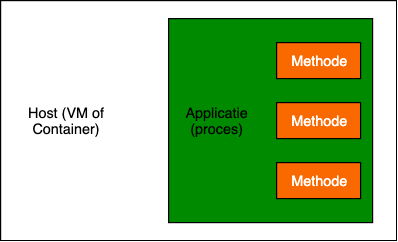
\includegraphics[width=0.7\textwidth]{img/traditional_software_deployment.png}
    \caption{Klassieke monoliet applicaties draaien als één proces op een besturingssysteem binnen een container of virtuele machine. Een klassieke applicatie is opgebouwd uit verschillende methoden met elk hun eigen functionaliteit gescheiden door softwareklassen.} 
    \label{fig:traditional-software-deployment}  
\end{figure}
\\
De FaaS benadering verandert het klassieke model van applicatie deployment. Ontwikkelaars schrijven in dit model individuele functies die losstaan van elkaar en elk hun eigen specifieke taak hebben. Een applicatie draait nu niet meer voortdurend in een VM of container maar de functionaliteit werkt event-driven. De functies die de ontwikkelaar schrijft worden opgeladen naar een FaaS platform. Omdat de applicatie niet meer voortdurend draait is het FaaS platform zo geconfigureerd dat het luistert naar events die gekoppeld zijn aan een specifieke functie. Wanneer er een event optreedt dat een functie aanroept dan zorgt het FaaS platform ervoor dat er een container wordt gestart, de code wordt ingeladen en uitgevoerd en na afloop van de functie wordt de container weer gestopt. Functies worden vaak aangeroepen aan de hand van HTTP API Gateway calls, in de voorbeelden die volgen wordt de cyclus van FaaS duidelijk weergegeven. Hoe dit nu serverless is? Wel , ontwikkelaars dienen zich enkel maar te focussen op het schrijven van code (functies) en deze plaatsen ze gewoon in het FaaS platform, zonder zorg over de achterliggende infrastructuur.\autocite{Roberts2017}
\\\\
Er zijn al heel wat cloud providers die Function-as-a-Service platforms aanbieden en de populairste op moment van schrijven zijn ongetwijfeld: Amazon Web Services met hun AWS Lambda, Google Cloud Platform met Google Cloud Functions en Microsoft Azure met Azure Functions. De opgesomde platformen zijn allen proprietary,  dit wilt zeggen dat ze gepatenteerd zijn en in bezit van een tech-gigant, en dus niet open source. De FaaS platformen die de grote spelers aanbieden zijn al ver ontwikkeld en bieden heel wat functionaliteit maar zullen niet verder behandeld worden in dit onderzoek. Als alternatief duiken er steeds meer en meer open source frameworks op voor het opzetten van een FaaS platform. In verder onderzoek zal een overweging worden gemaakt welke  open source frameworks het meest interessant zijn voor Nubera en die aan hun vereisten voldoen.

\subsection{Serverless concepten, begrippen en onderdelen}
Het begrip serverless zou nu al een stuk duidelijker moeten zijn. Serverless brengt echter nog meer begrippen mee om het volledige plaatje te kunnen schetsen. In deze sectie worden de belangrijkste ''key concepts'' met bijhorende begrippen nader verklaard.

\subsubsection{Next-Gen applicaties}
Applicaties die in een serverless omgeving draaien worden vaak next-gen applicaties genoemd. Met next-generation applicaties bedoelen we de applicaties die in een Cloud gebaseerde omgeving draaien en een onderliggende architectuur hebben die bestaat uit enerzijds containers en anderzijds microservices. Applicatieontwikkeling is de afgelopen 10 jaar enorm veranderd. Nu is het hele development gebeuren gericht op continue integratie en continue delivery (CI/CD) en zijn de ontwikkelingscyclussen (tijd tussen applicatie releases) verkleind van een aantal weken of aantal maanden tot een aantal minuten, uren of weken in het slechtste geval. 

\subsubsection{Microservices}
Microservices is een alternatief voor klassieke monoliet applicaties, dit zijn applicaties die verschillende functionaliteiten omvatten en draaien als een enkel proces binnen een VM of container. Een monoliet applicatie kan worden gezien als één gehele applicatie die draait op één machine.  In microservices daarentegen worden verschillende functionaliteiten en services gegroepeerd met elk hun eigen verantwoordelijkheden. Microservices zijn als het ware  een decompositie van een monoliet applicatie. Applicaties ontwikkeld volgens een microservices architectuur bestaan uit onafhankelijke componenten die naast elkaar bestaan en makkelijk vervangbaar of upgradebaar zijn. In een klassiek ontwerp van een applicatie is de applicatielogica van elkaar gescheiden door behulp van verschillende softwareklassen. De softwareklassen kunnen met elkaar communiceren. In een microservice architectuur kunnen de verschillende componenten ook met elkaar communiceren maar dit gebeurt aan de hand van REST API vaak via het HTTP protocol. Daar waar monoliet applicaties gebruik maken van eenzelfde datastore, zijn elk component van microservices verantwoordelijk voor hun eigen data en persistentie. Een microservice kan de data van een andere microservice niet rechtstreeks raadplegen. Verschillende microservices kunnen draaien in verschillende VMs of containers, daarom wordt deze architectuur ook wel loosely-coupled genoemd.\autocite{Fowler2014}

\subsubsection{Containers}
In essentie is een container te vergelijken met een zeer kleine VM. Volgens \textcite{Docker2019} is een container een stuk software dat alle code en dependencies van een applicatie omvat zodat een applicatie op eender welke computeromgeving hetzelfde draait. De container bevat alles dat een applicatie nodig heeft om naar behoren te kunnen werken, onder andere: code, runtime, systeem programma's zoals binaries, systeem libraries en instellingen. Een ontwikkelaar is in staat om zelf container samen te stellen die voldoet aan zijn/haar vereisten. Concreet kan een ontwikkelaar dus een container image maken en hieruit kan dan een container worden opgezet. Een container image en de container die daaruit wordt opgebouwd ziet er overal hetzelfde uit ongeacht het onderliggend systeem. Figuur \ref{fig:virtualisatie_vs_containers} toont het verschil in architectuur tussen een gevirtualiseerde infrastructuur en een infrastructuur waarin containers draaien.
 \begin{figure}
     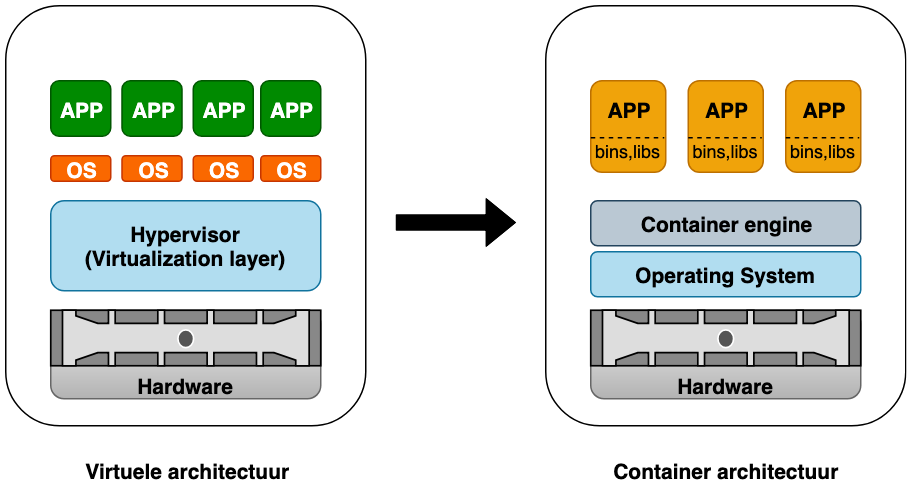
\includegraphics[width=1\textwidth]{img/virtualisatie_vs_containers.png}
     \caption{De figuur links weergeeft een representatie van een gevirtualiseerde architectuur. Rechts is er een gecontaineriseerde architectuur te zien. Bovenop de hardware en het besturingssysteem draait een container engine, de bekendste container engine is ongetwijfeld Docker engine. Bovenop de container engine draaien de containers met elk hun eigen binaries, libraries en applicatie.} 
     \label{fig:virtualisatie_vs_containers}  
 \end{figure}


\subsubsection{API Gateway}
Wanneer functies worden aangeroepen, dan gebeurt dat binnen FaaS vaak via een API gateway aan de hand van HTTP. Microservices communiceren ook met elkaar via deze API gateways, op die manier kunnen verschillende microservices gebruik maken van elkaars functionaliteit.
\textcite{Roberts2017} beschrijven de taak van een API gateway als die van een webserver die verantwoordelijk is voor het ontvangen en routeren van HTTP requests. Een request dat wordt ontvangen, wordt gerouteerd naar de handler gebaseerd op de route van de HTTP request. De API gateway ontvangt het antwoord van de handler en routeert dit uiteindelijk terug naar de originele client. Zoals eerder al aangehaald zijn handlers binnen FaaS infrastructuren vaak de functies geschreven door de ontwikkelaars. De API gateway is op de hoogte van alle handlers waar requests naar kunnen worden gerouteerd, deze worden meegegeven in de configuratie van de API. Figuur \ref{fig:api-gateway} geeft een schematische voorstelling van hoe een API gateway eruitziet.
 
 \begin{figure}
    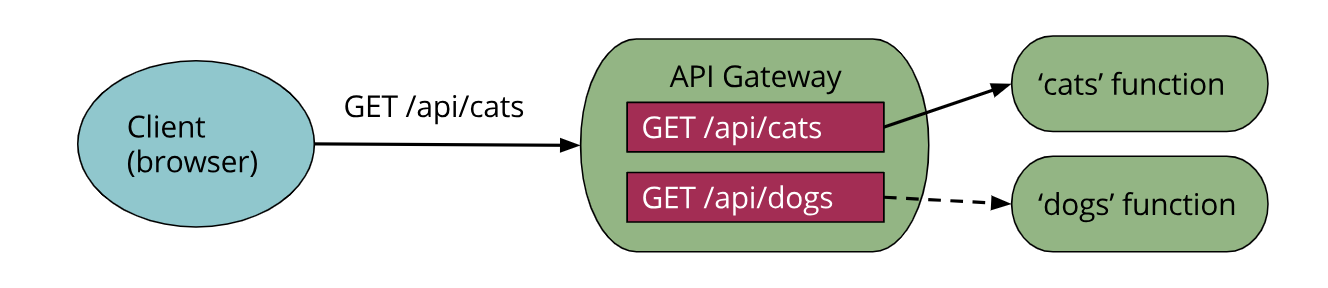
\includegraphics[width=1\textwidth]{img/api_gateway.png}
    \caption{In de figuur is een schematische voorstelling van het API gateway concept te zien. Wanneer een client (webbrowser) een HTTP GET request verstuurd naar het pad /api/cats, dan ontvangt de API gateway dit request en zoekt deze in zijn configuratie. Wanneer de handler is gevonden, wordt het GET request doorgestuurd naar de handler, in dit geval een functie genaamd ''cats''. De functie retourneert de opgevraagde inhoud naar de API gateway die het request op zijn beurt terugstuurt naar de originele client, in dit geval de webbrowser.\autocite{Roberts2018}} 
    \label{fig:api-gateway}  
\end{figure}

\subsection{Serverless architectuur}
Hoe serverless infrastructuren eruitzien wordt in deze sectie uitgelegd aan de hand van voorbeelden gebaseerd op een zeer interessant artikel over serverless computing door \textcite{Roberts2018}. Er worden twee voorbeelden aangehaald die kunnen dienen als richtlijnen voor verschillende soorten applicaties.

\subsubsection{Applicaties met een user-interface}
In dit voorbeeld bestaat de architectuur uit de klassieke drie-lagen benadering. Er is een client systeem, in dit geval een webbrowser, een server met serverlogica en applicatiecode en een achterliggende databank voor persistentie. De gehanteerde benadering zorgt ervoor dat de client van niets op de hoogte is en dat alle logica aanwezig is in het systeem. De applicatieserver is verantwoordelijk voor alle functionaliteiten zoals: authenticatie, navigatie, zoekmogelijkheden en transacties. In figuur \ref{fig:drielagen_architectuur} wordt de architectuur schematisch voorgesteld.
\begin{figure}
    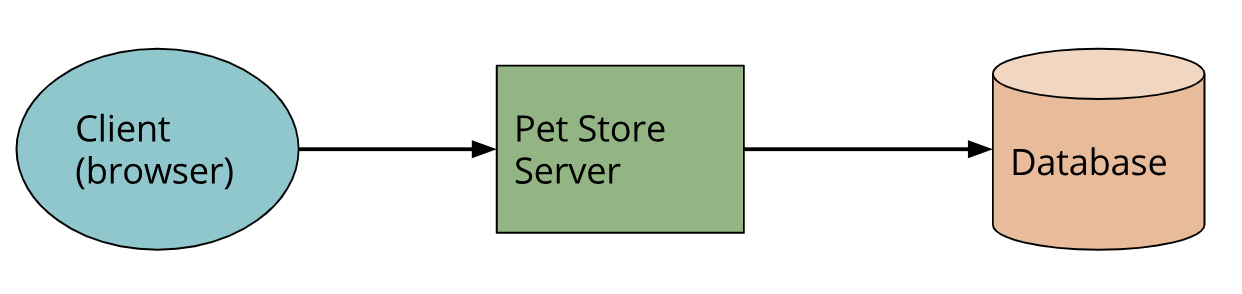
\includegraphics[width=1\textwidth]{img/drielagen_architectuur.png}
    \caption{De figuur weergeeft een schematische voorstelling van een  applicatie opgebouwd volgens het drie-lagen model. De client fungeert enkel als grafische interface en bevat niets van achterliggende code. De applicatieserver bevat alle applicatielogica en maakt gebruik van een achterliggend databanksysteem. \autocite{Roberts2018}} 
    \label{fig:drielagen_architectuur}  
\end{figure}
\\\\
Wanneer de klassieke benadering wordt omgevormd volgens een serverless architectuur, dan wordt de applicatie op een volledig andere manier ontwikkeld zodanig dat nu ook de client verantwoordelijkheden heeft en alles niet afhankelijk is van één enkele applicatieserver. Figuur \ref{fig:serverless_architectuur} geeft een overzicht van de opbouw van de applicatie in een serverless omgeving.
\begin{figure}
    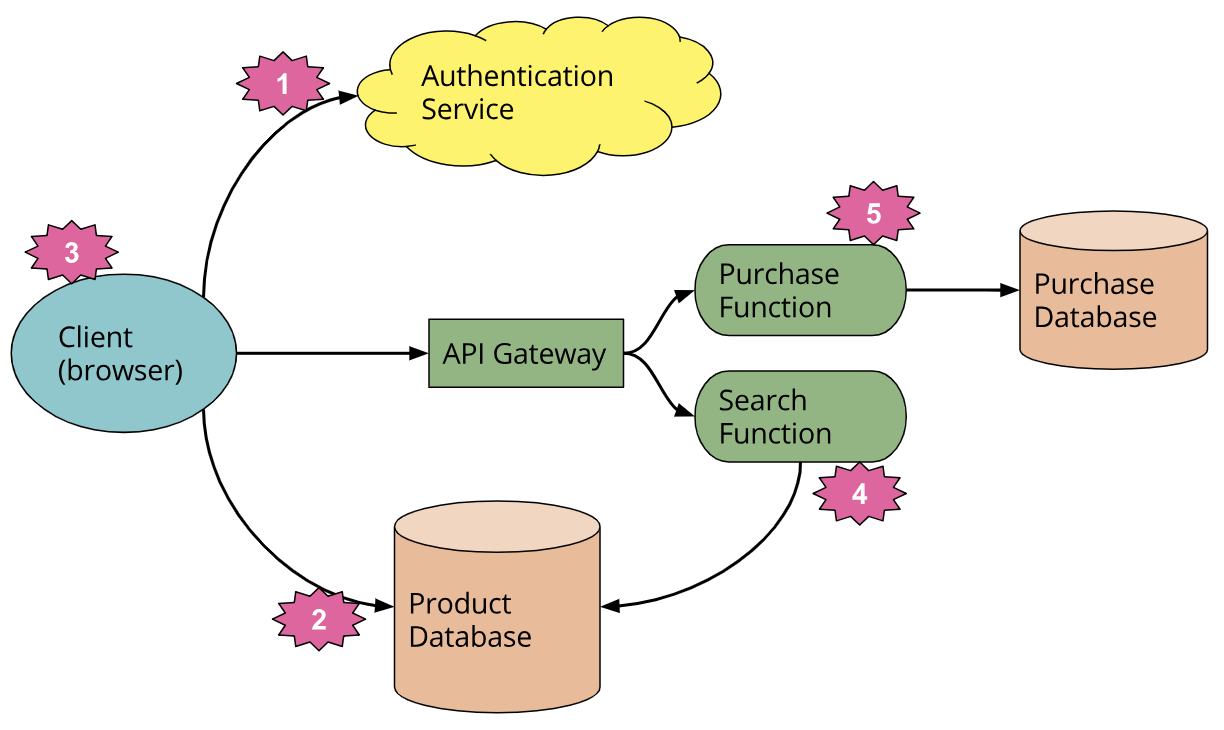
\includegraphics[width=1\textwidth]{img/serverless_architectuur.png}
    \caption{De figuur weergeeft een schematische voorstelling van een applicatie die opgebouwd is volgens een serverless architectuur. De applicatielogica wordt opgesplitst in verschillende microservices met elk hun eigen functionaliteit. \autocite{Roberts2018}} 
    \label{fig:serverless_architectuur}  
\end{figure}
In de figuur zijn onmiddellijk enkele grote verschillen te bemerken in vergelijking met de klassieke drie-lagen architectuur zoals in figuur \ref{fig:drielagen_architectuur}:
\begin{enumerate}
    \item De authenticatie logica die initieel verwerkt was in de applicatie op de applicatieserver is verplaatst uit de applicatie en wordt vervangen door een Backend-as-a-Service dienst die wordt aangeboden door een derde partij, bijvoorbeeld Okta.
    \item De databank die eerst enkel raadpleegbaar was door de applicatieserver is nu ook te bereiken door de client. De databank wordt uitbesteed aan een derde partij alweer als BaaS dienst, een mogelijkheid hiervoor is Google Firebase zoals eerder in dit onderzoek al werd aangehaald.
    \item De voorgaande twee stappen zorgen ervoor dat de applicatielogica die initieel enkel beschikbaar was binnen de applicatieserver, nu ook beschikbaar is via de client. De client maakt op deze manier de transitie van ''domme'' component in het gehele verhaal, naar een intelligent deel software dat op de hoogte is van verschillende applicatieonderdelen. De client evolueert in de richting van een ''Single Page Application''. 
    \item De applicatie heeft nog steeds nood aan toegang tot de databank voor het ophalen en wegschrijven van records. In plaats van het hebben van een server die voortdurend staat de draaien om records te kunnen opvragen, wordt deze functionaliteit in een serverless architectuur vervangen door een functie. Een functie fungeert als handler die luistert op requests die via de API gateway worden gerouteerd. In dit voorbeeld luistert een functie ''search'' naar binnenkomende HTTP requests. De functie heeft toegang tot de databank dienst die door een derde partij onderhouden wordt.
    \item In de laatste stap wordt er ook een functie gebruikt voor de ''purchase'' functionaliteit. Er wordt opnieuw geopteerd om de functie te implementeren in de server-side kant voor veiligheidsmaatregelen. Het is gebruikelijk dat een applicatie wordt opgesplits in verschillende functies met elk hun eigen functionaliteit in een FaaS omgeving.
\end{enumerate}

De serverless benadering volgt dezelfde als deze van microservices zoals eerder behandeld. Een klassieke monoliet applicatie wordt opgesplitst in verschillende onderdelen met elk hun eigen functionaliteit, dit kunnen enerzijds BaaS componenten zijn, anderzijds FaaS functies. Zoals het voorbeeld vast al aangeeft, biedt een serverless architectuur enorm veel flexibiliteit en mogelijkheden. Werken volgens een serverless infrastructuur stelt teams in staat om individueel te werken aan kleine onderdelen van een applicatie, zo kan er bijvoorbeeld voor elke functie een klein team de verantwoordelijkheid dragen. Het is misschien ook al opgevallen dat de ontwikkelaars niet meer bezig hoeven te zijn met servers zelf maar enkel met code zelf. FaaS frameworks zorgen ervoor dat de overhead van achterliggende servers volledig wordt weggenomen en dat de focus enkel en alleen op code ligt.

\subsubsection{Bericht gedreven applicaties}
Een veelvoorkomend voorbeeld dat ook werkt volgens een FaaS architectuur is een service voor backend data-processing. Neem bijvoorbeeld een online advertentie systeem, welbekende advertenties die overal terug te vinden zijn op websites. Wanneer een gebruiker op een advertentie klikt moet hij naar de juiste website worden doorgestuurd en moet het click-event worden opgeslagen zodat de het advertentiesysteem de adverteerder kan aanrekenen.
Klassiek zou zo'n architectuur eruitzien zoals in figuur \ref{fig:klassiek-message-driven}. De Ad Server luistert naar wanneer er een gebruiker op een advertentie klikt, in dat geval post de Ad Server een ''Click message'' in een bericht channel. Het geposte bericht wordt op zijn beurt door een Click Processor verwerkt die instaat voor het bijwerken van de databank, het aanrekenen van de adverteerder etc.
\begin{figure}
    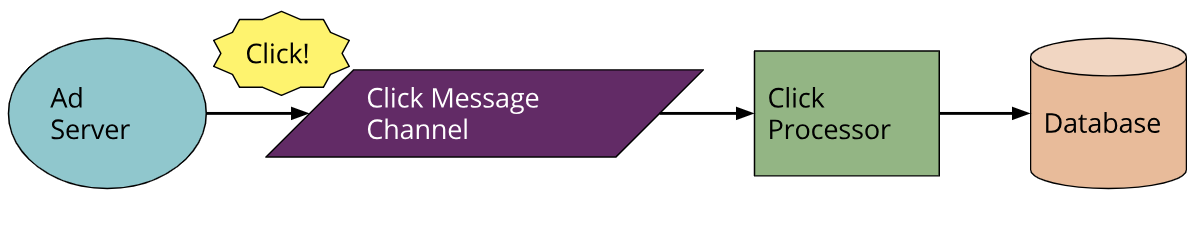
\includegraphics[width=1\textwidth]{img/klassiek_message_driven.png}
    \caption{De figuur weergeeft een schematische voorstelling van een message-driven applicatie van een advertentie systeem opgezet volgens klassieke benadering met alle code in één enkele applicatie. \autocite{Roberts2018}} 
    \label{fig:klassiek-message-driven}  
\end{figure}

Wanneer de applicatie wordt omgevormd naar een serverless architectuur dan is in figuur \ref{fig:faas-message-driven} te zien dat een volledige click processor applicatie vervangen is door verschillende FaaS functies die elk hun eigen functionaliteit hebben. De functies zijn event-driven en worden uitgevoerd op het moment dat er een click message ontvangen wordt. De cloud provider (in geval van een on-premises of private cloud oplossing, het serverless framework)  voorziet zowel de FaaS omgeving als het systeem dat de berichten ontvangt.
\begin{figure}
    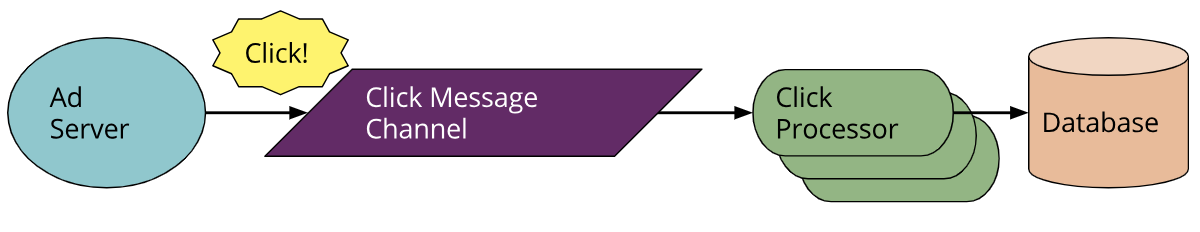
\includegraphics[width=1\textwidth]{img/faas_message_driven.png}
    \caption{De figuur weergeeft een schematische voorstelling van een message-driven applicatie van een advertentie systeem geschreven specifiek voor een FaaS omgeving. De applicatie is opgesplitst in verschillende functies met elk hun eigen functionaliteit. \autocite{Roberts2018}} 
    \label{fig:faas-message-driven}  
\end{figure}

\subsection{Serverless voor-en nadelen}
Zoals reeds al enkele keren werd aangehaald biedt een serverless architectuur voor applicaties heel wat voordelen ten opzichte van de klassieke benadering voor applicatieontwikkeling. Echter zijn de nadelen ook niet over het hoofd te zien, deze dienen bestudeerd te worden door iedereen die overweegt om de transitie richting serverless applicaties te maken. \textcite{Stigler2017} beschrijft zowel voor- en nadelen die het meest terugkomen bij het lezen over serverless architecturen.

\subsubsection{Voordelen}

\begin{description}[style=unboxed, labelwidth=\linewidth, listparindent =0pt]
    \item[Geen beheer van infrastructuur]
    Voor ontwikkelaars is het interessant dat ze zich niet meer hoeven te focussen op het beheer van achterliggende servers en databanksystemen waarop applicaties draaien. Een ontwikkelaar hoeft zich enkel nog te focussen op de logica, de code die hij schrijft.
    \newline
    
    \item [Snellere development en deployment]
    Omdat de ontwikkelaars niet meer bezig moeten zijn met de servers kunnen ze zich meer focussen op het schrijven van code waardoor het development proces sneller verloopt. Daarnaast is het mogelijk, wanneer de FaaS omgeving draait bij een van de grote cloud spelers, gebruik te maken van functie templates waardoor code onmiddellijk kan worden uitgevoerd.
    \newline
    
    \item [Makkelijk in gebruik]
    Zowel grote cloud providers die serverless oplossingen aanbieden, als open source alternatieven zijn zo ontwikkeld dat het bouwen van FaaS applicaties vrij makkelijk is. Providers en frameworks bieden vaak alle componenten aan die een ontwikkelaar nodig heeft voor het bouwen van een applicatie, van API gateway tot object opslag waar functies gebruik van maken om data op te halen of weg te schrijven. Het enige dat de ontwikkelaar hoeft te doen is de componenten configureren, de code schrijven en uploaden.
    \newline
    
    \item [Lagere kosten]
    Bij gebruik van een FaaS infrastructuur betaal je een prijs per functie die wordt uitgevoerd, in het geval de applicatie gehost wordt bij een publieke cloud provider. Wanneer je een serverless infrastructuur draait in een eigen datacenter dan betaal je natuurlijk niet minder want je moet nog steeds servers aankopen, hoewel het wel mogelijk is om minder resources te verbruiken omdat serverless functies per code executie opnieuw een container te starten en deze na afloop ook weer verwijderen. In een private setting is het dus wel zo dat er een lagere kost is op basis van resources.
    \newline
    
     \item [Verbeterde schaalbaarheid]
     Wanneer de FaaS inrastructuur draait bij een grote cloud provider dan is er meestal automatische schaalbaarheid beschikbaar, een ontwikkelaar hoeft zich hierover dus geen zorgen te maken. Wanneer de infrastructuur draait in een eigen datacenter dan kan deze schaalbaarheid ook voorzien worden aan de hand van een functie die vooraf wordt gedefinieerd en vervolgens schaalbaarheid zal voorzien.
     \newline 
\end{description}

\subsubsection{Nadelen of beperkingen}

\begin{description}[style=unboxed, labelwidth=\linewidth, listparindent =0pt]
    \item[Geen controle over infrastructuur]
    Bij het gebruik van cloud diensten van grote cloud spelers is de controle over achterliggend systeem beperkt. De ontwikkelaar heeft de mogelijkheid voor het kiezen van computing resources, permissies en timeout, verder onderhoud van de systemen is afgeschermd voor ontwikkelaars.
    \newline
    
    \item[Server applicatie die lang draait]
    Sommige applicaties die gebruikmaken van batch-processing draaien soms erg lang. Serverless architecturen zijn net zo ontworpen om snel, schaalbaar en event-driven te zijn en daarbinnen passen batch processing applicaties niet meteen. Serverless biedt echter wel mogelijkheden dat soort applicaties om te vormen naar een FaaS applicatie.
    \newline
    
     \item[Vendor lock-in]
     Wanneer bedrijven opteren om bijvoorbeeld gebruik te maken van AWS Lambda, dan zitten ze hieraan vast en is het moeilijk om hiervan weg te stappen wegens de grote moeite en kost die migratie naar de cloud met zich meebrengt. Er bestaan echter al alternatieven die ervoor zorgen dat functies werken ongeacht de onderliggende provider. Een populaire benadering is om de logica uit cloud-specifieke handlers te halen en deze te configureren in een framework dat werkt voor verschillende cloud providers, bijvoorbeeld Serverless Framework \autocite{Serverless2018}. De cloud provider logica wegnemen uit de event handler maakt een applicatie herbruikbaar bij verschillende providers en biedt ook verhoogde flexibiliteit.
     \newline
     
     \item[Cold start]
     Het probleem met cold starts is vaak dat een functie extra tijd nodig heeft voor uitvoering in geval van een langere periode van inactiviteit. Grote cloud providers die serverless diensten aanbieden hebben voor dit probleem een oplossing. Wanneer functies maar om de zoveel tijd worden aangeroepen kan er gebruik worden gemaakt van schedulers die de functie op vaste tijdstippen aanroept, op die manier ondervindt de functie geen cold start en is er geen vertraging bij uitvoering. Een cold start is ook onderhevig aan de hoeveelheid memory van een systeem en de runtime, een applicatie geschreven in Java of C\# hebben een cold start die veel langer duurt in tegenstelling tot talen zoals Node.js  of Python.  Hoe meer memory aanwezig, hoe langer de cold start zal duren, meer memory heeft dus een nadelige invloed op de uitvoeringstijd.
\end{description}

\section{Grote spelers of trends in ontwikkeling?}
In dit hoofdstuk werd eerst de theorie omtrent cloud computing behandelt. Vervolgens werd aan de hand van voorbeelden en schematische voorstellingen het serverless concept uitgelegd. Het valt misschien op dat er vaak gerefereerd werd naar de grote spelers, zoals Amazon, Google, Microsoft of IBM. Momenteel bieden deze grote cloud providers al heel wat diensten aan om serverless te kunnen werken, deze services hebben allen voor- en nadelen zoals eerder behandeld werd. Er zijn veel bedrijven die worden afgeschrikt door de cloud omdat ze genoodzaakt lijken klant te worden bij een van deze grote spelers. De terughoudendheid heeft vaak te maken met argwaan omtrent databeveiliging en integriteit. Bedrijven die deze redenering volgen kunnen we geen ongelijk geven, wanneer het budget het toelaat is het nog steeds zeer interessant om een eigen datacenter op te zetten en te configureren als een private cloud omgeving. Sommige bedrijven met een private cloud of on-premises infrastructuur die interesse hebben in serverless infrastructuur kunnen hier ook mee naar evolueren zonder te moeten migreren naar de publieke cloud. Momenteel zijn er al heel wat open source alternatieven om serverless te werken. Open source tools laten het toe een eigen serverless infrastructuur op te zetten op locatie of in de private cloud gelijkaardig aan de serverless diensten die cloud providers aanbieden. In volgend hoofdstuk wordt er een alternatief open source framework gekozen voor Fission, hiervan wordt ook een Proof of Concept opgesteld. De tool wordt geselecteerd op basis van requirements opgesteld door Nubera, het bedrijf waarvoor deze bachelorproef wordt geschreven.

